\documentclass[english]{SPFShortReport}
\usepackage{subfigure}
\usepackage{spfFigures}
\usepackage{longtable}
\usepackage{url}
\usepackage{gensymb}
\usepackage[yyyymmdd,hhmmss]{datetime}
\reportName{Python calculation for heat pump SI-108-HT}
\reportSubName{Parametric Heat Pump calculation} 
\reportDate{\today \hspace{0.1cm} at: \currenttime \hspace{0.1cm} h} 
\author{Dani Carbonell}
\address{dani.carbonell@solarenergy.ch}
\begin{document}
\begin{table}[!ht]
\begin{small}
\caption{Fitted coefficients for the heat pump.}
\begin{center}
\resizebox{12cm}{!} 
{
\begin{tabular}{l | c c } 
\hline
\hline
Coefficient &Description & \\ 
 & &$[kW]$\\ 
\hline
$PQ_{1}$ & \emph{$1^{st}$ condenser polynomial coefficient}  & 1.1592e+01    \\ 
$PQ_{2}$ & \emph{$2^{st}$ condenser polynomial coefficient}  & 1.4291e+02    \\ 
$PQ_{3}$ & \emph{$3^{st}$ condenser polynomial coefficient}  & -2.9978e+01    \\ 
$PQ_{4}$ & \emph{$4^{st}$ condenser polynomial coefficient}  & -5.0425e+02    \\ 
$PQ_{5}$ & \emph{$5^{st}$ condenser polynomial coefficient}  & 5.0221e+02    \\ 
$PQ_{6}$ & \emph{$6^{st}$ condenser polynomial coefficient}  & 6.3589e+01    \\ 
\hline
$PCOP_{1}$ & \emph{$1^{st}$ COP polynomial coefficient}  & 1.0349e+01    \\ 
$PCOP_{2}$ & \emph{$2^{st}$ COP polynomial coefficient}  & 1.1188e+02    \\ 
$PCOP_{3}$ & \emph{$3^{st}$ COP polynomial coefficient}  & -5.9716e+01    \\ 
$PCOP_{4}$ & \emph{$4^{st}$ COP polynomial coefficient}  & -4.9672e+02    \\ 
$PCOP_{5}$ & \emph{$5^{st}$ COP polynomial coefficient}  & 5.0264e+02    \\ 
$PCOP_{6}$ & \emph{$6^{st}$ COP polynomial coefficient}  & 1.0878e+02    \\ 
\hline
$\dot m_{cond}$ & 900.00 $[kg/h]$\\ 
$\dot m_{evap}$ & 900.00 $[kg/h]$\\ 
\hline
$COP_{nom}$ (B0W35)& 4.37 \\ 
$Q_{c,nom}$ (B0W35)& 8.05 kW\\ 
$COP_{nom}$ (B2W35)& 4.69 \\ 
$Q_{c,nom}$ (B2W35)& 8.55 kW\\ 
$COP_{nom}$ (B10W35)& 6.40 \\ 
$Q_{c,nom}$ (B10W35)& 10.92 kW\\ 
\hline
\hline
\end{tabular}
}
\label{CoefTable}
\end{center}
\end{small}
\end{table}
\begin{table}[!ht]
\begin{small}
\caption{Predicting results of the heat pump.}
\begin{center}
\resizebox{12cm}{!} 
{
\begin{tabular}{l | c c c c c c c c c c c } 
\hline
\hline
$T_{evap,in}$ &$T_{evap,out}$ &$T_{cond,in}$ &$T_{cond,out}$ &$COP$ &$Q_{cond}$ &$Q_{evap}$ &$W_{comp}$ &$\dot m_{cond}$ &$\dot m_{evap}$ &$\Delta T_{evap}$ &$\Delta T_{cond}$ \\ 
$^oC$ &$^oC$ &$^oC$ &$^oC$ &$[-]$ &$[kW]$ &$[kW]$ &$[kW]$ &kg/h &kg/h &K &K\\ 
\hline
-7.00 & -12.16 & 23.70 & 30.00 & 3.94 & 6.60 & 4.93 & 1.68 & 900 & 900 & 5.2 & 6.3\\ 
-7.00 & -11.94 & 32.36 & 38.75 & 3.39 & 6.69 & 4.72 & 1.98 & 900 & 900 & 4.9 & 6.4\\ 
-7.00 & -11.85 & 40.92 & 47.50 & 3.05 & 6.89 & 4.63 & 2.26 & 900 & 900 & 4.8 & 6.6\\ 
-7.00 & -11.97 & 49.38 & 56.25 & 2.93 & 7.20 & 4.74 & 2.46 & 900 & 900 & 5.0 & 6.9\\ 
-7.00 & -12.38 & 57.70 & 65.00 & 3.05 & 7.65 & 5.14 & 2.51 & 900 & 900 & 5.4 & 7.3\\ 
-4.00 & -9.81 & 23.10 & 30.00 & 4.29 & 7.23 & 5.54 & 1.69 & 900 & 900 & 5.8 & 6.9\\ 
-4.00 & -9.42 & 31.90 & 38.75 & 3.58 & 7.17 & 5.17 & 2.00 & 900 & 900 & 5.4 & 6.8\\ 
-4.00 & -9.11 & 40.61 & 47.50 & 3.07 & 7.22 & 4.87 & 2.35 & 900 & 900 & 5.1 & 6.9\\ 
-4.00 & -8.95 & 49.21 & 56.25 & 2.78 & 7.38 & 4.72 & 2.66 & 900 & 900 & 4.9 & 7.0\\ 
-4.00 & -9.05 & 57.70 & 65.00 & 2.70 & 7.64 & 4.82 & 2.83 & 900 & 900 & 5.0 & 7.3\\ 
-1.00 & -7.57 & 22.42 & 30.00 & 4.74 & 7.94 & 6.27 & 1.68 & 900 & 900 & 6.6 & 7.6\\ 
-1.00 & -7.03 & 31.35 & 38.75 & 3.88 & 7.75 & 5.75 & 2.00 & 900 & 900 & 6.0 & 7.4\\ 
-1.00 & -6.53 & 40.19 & 47.50 & 3.22 & 7.66 & 5.28 & 2.38 & 900 & 900 & 5.5 & 7.3\\ 
-1.00 & -6.12 & 48.93 & 56.25 & 2.76 & 7.67 & 4.89 & 2.78 & 900 & 900 & 5.1 & 7.3\\ 
-1.00 & -5.89 & 57.58 & 65.00 & 2.50 & 7.77 & 4.66 & 3.11 & 900 & 900 & 4.9 & 7.4\\ 
2.00 & -5.43 & 21.65 & 30.00 & 5.29 & 8.75 & 7.09 & 1.65 & 900 & 900 & 7.4 & 8.4\\ 
2.00 & -4.77 & 30.71 & 38.75 & 4.28 & 8.42 & 6.45 & 1.97 & 900 & 900 & 6.8 & 8.0\\ 
2.00 & -4.11 & 39.68 & 47.50 & 3.47 & 8.19 & 5.83 & 2.36 & 900 & 900 & 6.1 & 7.8\\ 
2.00 & -3.49 & 48.56 & 56.25 & 2.85 & 8.06 & 5.24 & 2.82 & 900 & 900 & 5.5 & 7.7\\ 
2.00 & -2.95 & 57.35 & 65.00 & 2.43 & 8.02 & 4.72 & 3.30 & 900 & 900 & 4.9 & 7.7\\ 
5.00 & -3.40 & 20.80 & 30.00 & 5.93 & 9.64 & 8.01 & 1.62 & 900 & 900 & 8.4 & 9.2\\ 
5.00 & -2.61 & 29.98 & 38.75 & 4.78 & 9.18 & 7.26 & 1.92 & 900 & 900 & 7.6 & 8.8\\ 
5.00 & -1.83 & 39.08 & 47.50 & 3.83 & 8.82 & 6.52 & 2.31 & 900 & 900 & 6.8 & 8.4\\ 
5.00 & -1.04 & 48.09 & 56.25 & 3.06 & 8.55 & 5.76 & 2.79 & 900 & 900 & 6.0 & 8.2\\ 
5.00 & -0.24 & 57.01 & 65.00 & 2.48 & 8.37 & 5.00 & 3.37 & 900 & 900 & 5.2 & 8.0\\ 
8.00 & -1.46 & 19.86 & 30.00 & 6.67 & 10.62 & 9.03 & 1.59 & 900 & 900 & 9.5 & 10.1\\ 
8.00 & -0.56 & 29.17 & 38.75 & 5.38 & 10.03 & 8.17 & 1.86 & 900 & 900 & 8.6 & 9.6\\ 
8.00 & 0.34 & 38.39 & 47.50 & 4.28 & 9.54 & 7.31 & 2.23 & 900 & 900 & 7.7 & 9.1\\ 
8.00 & 1.26 & 47.53 & 56.25 & 3.37 & 9.14 & 6.43 & 2.71 & 900 & 900 & 6.7 & 8.7\\ 
8.00 & 2.24 & 56.58 & 65.00 & 2.65 & 8.82 & 5.49 & 3.33 & 900 & 900 & 5.8 & 8.4\\ 
11.00 & 0.39 & 18.85 & 30.00 & 7.50 & 11.68 & 10.12 & 1.56 & 900 & 900 & 10.6 & 11.1\\ 
11.00 & 1.40 & 28.28 & 38.75 & 6.07 & 10.97 & 9.16 & 1.81 & 900 & 900 & 9.6 & 10.5\\ 
11.00 & 2.40 & 37.62 & 47.50 & 4.83 & 10.34 & 8.20 & 2.14 & 900 & 900 & 8.6 & 9.9\\ 
11.00 & 3.44 & 46.88 & 56.25 & 3.78 & 9.81 & 7.22 & 2.59 & 900 & 900 & 7.6 & 9.4\\ 
11.00 & 4.55 & 56.06 & 65.00 & 2.92 & 9.37 & 6.15 & 3.21 & 900 & 900 & 6.5 & 8.9\\ 
14.00 & 2.16 & 17.76 & 30.00 & 8.42 & 12.82 & 11.30 & 1.52 & 900 & 900 & 11.8 & 12.2\\ 
14.00 & 3.27 & 27.31 & 38.75 & 6.86 & 11.99 & 10.24 & 1.75 & 900 & 900 & 10.7 & 11.4\\ 
14.00 & 4.37 & 36.77 & 47.50 & 5.48 & 11.24 & 9.19 & 2.05 & 900 & 900 & 9.6 & 10.7\\ 
14.00 & 5.50 & 46.16 & 56.25 & 4.29 & 10.57 & 8.11 & 2.47 & 900 & 900 & 8.5 & 10.1\\ 
14.00 & 6.71 & 55.46 & 65.00 & 3.28 & 10.00 & 6.95 & 3.05 & 900 & 900 & 7.3 & 9.5\\ 
17.00 & 3.84 & 16.60 & 30.00 & 9.43 & 14.04 & 12.55 & 1.49 & 900 & 900 & 13.2 & 13.4\\ 
17.00 & 5.05 & 26.25 & 38.75 & 7.73 & 13.09 & 11.40 & 1.69 & 900 & 900 & 11.9 & 12.5\\ 
17.00 & 6.25 & 35.84 & 47.50 & 6.22 & 12.22 & 10.25 & 1.96 & 900 & 900 & 10.7 & 11.7\\ 
17.00 & 7.47 & 45.34 & 56.25 & 4.89 & 11.43 & 9.09 & 2.34 & 900 & 900 & 9.5 & 10.9\\ 
17.00 & 8.77 & 54.77 & 65.00 & 3.74 & 10.72 & 7.86 & 2.86 & 900 & 900 & 8.2 & 10.2\\ 
20.00 & 5.45 & 15.36 & 30.00 & 10.52 & 15.34 & 13.88 & 1.46 & 900 & 900 & 14.5 & 14.6\\ 
20.00 & 6.76 & 25.12 & 38.75 & 8.69 & 14.27 & 12.63 & 1.64 & 900 & 900 & 13.2 & 13.6\\ 
20.00 & 8.06 & 34.82 & 47.50 & 7.05 & 13.28 & 11.40 & 1.88 & 900 & 900 & 11.9 & 12.7\\ 
20.00 & 9.36 & 44.45 & 56.25 & 5.58 & 12.36 & 10.15 & 2.21 & 900 & 900 & 10.6 & 11.8\\ 
20.00 & 10.73 & 53.99 & 65.00 & 4.30 & 11.53 & 8.85 & 2.68 & 900 & 900 & 9.3 & 11.0\\ 
\hline
\hline
\end{tabular}
}
\label{ResultsTable}
\end{center}
\end{small}
\end{table}
\begin{figure}[!ht]
\begin{center}
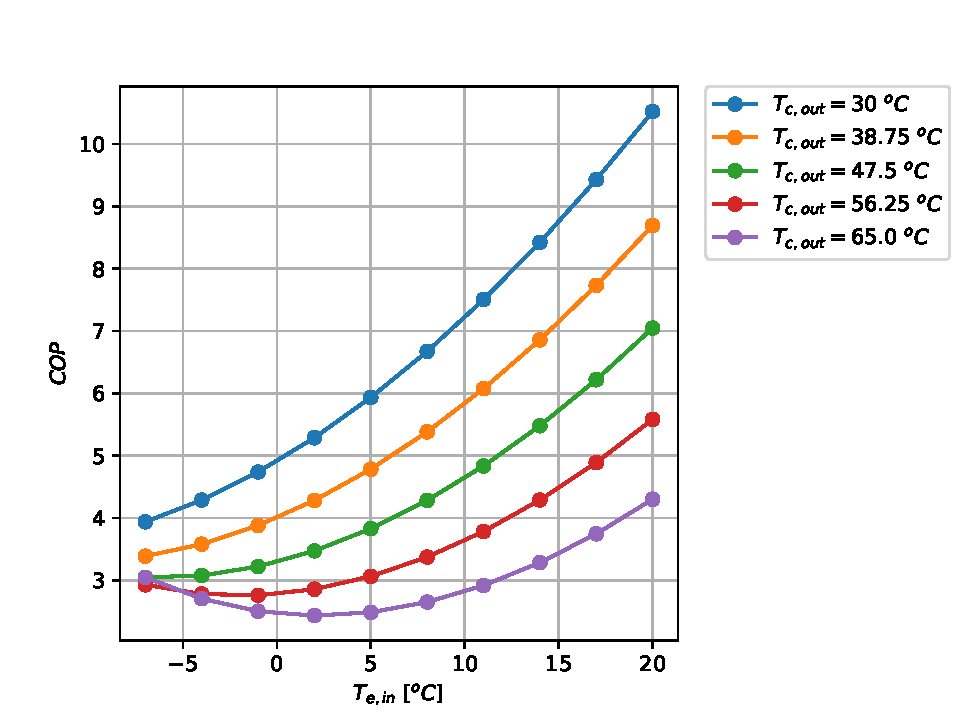
\includegraphics[width=1\textwidth]{C:/Daten/spfPackages/GIT/spfTrnsysFiles/HeatPump/BrineToWater/Walter Meier/SI-108-HT/SI-108-HT-Cop.pdf}
\caption{COP Results for the heat pump at the selected points}
\label{COPFig}
\end{center}
\end{figure}
\begin{figure}[!ht]
\begin{center}
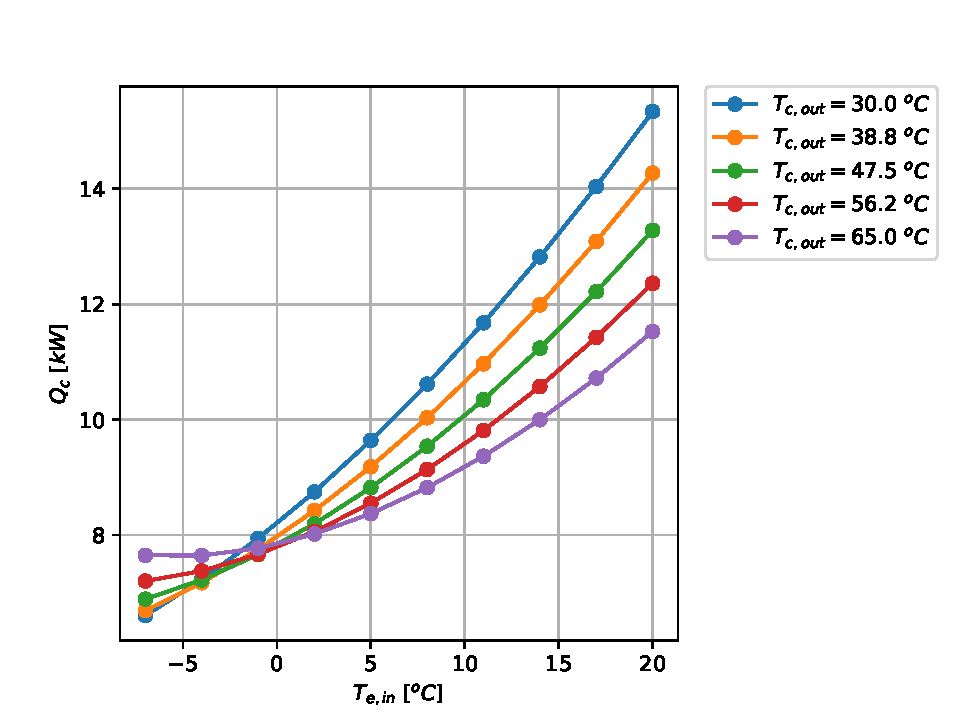
\includegraphics[width=1\textwidth]{C:/Daten/spfPackages/GIT/spfTrnsysFiles/HeatPump/BrineToWater/Walter Meier/SI-108-HT/SI-108-HT-Qc.pdf}
\caption{$Q_c$ Results for the heat pump at the selected points}
\label{QcFig}
\end{center}
\end{figure}
\end{document}
